\documentclass{beamer}
%\documentclass[17pt]{beamer}
%**********************************************************************************************************************************************
\usepackage{multicol, stmaryrd, amsfonts, graphicx, times, epsfig, amsmath, mathtools, subfigure, balance, array, siunitx, pgfgantt, xspace, graphicx, pgf, animate, algorithmic, algorithm, svg}
\usepackage{multirow, epsf, amsmath, amssymb, indentfirst, verbatim, keyval, url, textcomp, enumerate, calc, makecell, subfigure, xcolor, listings}
%**********************************************************************************************************************************************
\usepackage[utf8]{inputenc}
\usepackage[export]{adjustbox}
%\usepackage[absolute,overlay]{textpos}
\usepackage{hyperref}
\usepackage[normalem]{ulem}
\usepackage{textpos}
%**********************************************************************************************************************************************
\useunder{\uline}{\ulined}{}%
\DeclareUrlCommand{\bulurl}{\def\UrlFont{\ttfamily\color{blue}\ulined}}
\usefonttheme{serif}
\usetheme{Pittsburgh}
\usecolortheme{seahorse}
\graphicspath{ {figs/} }
\setbeamertemplate{itemize items}[ball]
\setbeamertemplate{bibliography item}[text]
\hypersetup{
   colorlinks   = true,                               %Colours links instead of ugly boxes
   urlcolor     = blue,                               %Colour for external hyper links
   linkcolor    = blue,                               %Colour of internal links
   citecolor    = red,                                %Colour of citations
   setpagesize  = false,
   linktocpage  = true,
}
%**********************************************************************************************************************************************
%\usepackage{stmaryrd, amsfonts, graphicx, times, epsfig, amsmath, mathtools,subfigure, balance, array,siunitx}
%\usefonttheme{structuresmallcapsserif}
%\usepackage{bookman}
%\usetheme{Madrid}
%\usetheme{Szeged}
%**********************************************************************************************************************************************
 \AtBeginSection[]
{
  \begin{frame}
    \frametitle{Table of Contents}
    \tableofcontents[currentsection]
  \end{frame}
}
%**********************************************************************************************************************************************
%\author[Arthur, Doe] % (optional, for multiple authors)
%{A.~B.~Arthur\inst{1} \and J.~Doe\inst{2}}
%
%\institute[VFU] % (optional)
%{
%  \inst{1}%
%  Faculty of Physics\\
%  Very Famous University
%  \and
%  \inst{2}%
%  Faculty of Chemistry\\
%  Very Famous University
%}
%**********************************************************************************************************************************************
\date[] % (optional)

%\logo{
\includegraphics[width=1in, height=0.3in]{GW_logo.eps}}
\titlegraphic{
\includegraphics[width=2in, height=0.8in]{GNN/imgs/GW_logo-eps-converted-to.pdf}}
%>>>>>>>>>>>>>>>>>>>>>>>>>>>>>>>>>>>>>>>>>>>>>>>>>>>>>>>>>>>>>>>>>>>>>>>>>>>>>>>>>>>>>>>>>>>>>>>>>>>>>>>>>>>>>>>>>>>>>>>>>>>>>>>>>>>>>>>>>>>>>>>
%>>>>>>>>>>>>>>>>>>>>>>>>>>>>>>>>>>>>>>>>>>>>>>>>>>>>>>>>>>>>>>>>>>>>>>>>>>>>>>>>>>>>>>>>>>>>>>>>>>>>>>>>>>>>>>>>>>>>>>>>>>>>>>>>>>>>>>>>>>>>>>>\setbeamertemplate{bibliography item}[text]

\usepackage{setspace}
\definecolor{Code}{rgb}{0,0,0}
\definecolor{Decorators}{rgb}{0.5,0.5,0.5}
\definecolor{Numbers}{rgb}{0.5,0,0}
\definecolor{MatchingBrackets}{rgb}{0.25,0.5,0.5}
\definecolor{Keywords}{rgb}{0,0,1}
\definecolor{self}{rgb}{0,0,0}
\definecolor{Strings}{rgb}{0,0.63,0}
\definecolor{Comments}{rgb}{0,0.63,1}
\definecolor{Backquotes}{rgb}{0,0,0}
\definecolor{Classname}{rgb}{0,0,0}
\definecolor{FunctionName}{rgb}{0,0,0}
\definecolor{Operators}{rgb}{0,0,0}
\definecolor{Background}{rgb}{0.98,0.98,0.98}
\lstdefinelanguage{Python}{
numbers=left,
numberstyle=\footnotesize,
numbersep=1em,
xleftmargin=1em,
framextopmargin=2em,
framexbottommargin=2em,
showspaces=false,
showtabs=false,
showstringspaces=false,
frame=l,
tabsize=4,
% Basic
basicstyle=\ttfamily\small\setstretch{1},
backgroundcolor=\color{Background},
% Comments
commentstyle=\color{Comments}\slshape,
% Strings
stringstyle=\color{Strings},
morecomment=[s][\color{Strings}]{"""}{"""},
morecomment=[s][\color{Strings}]{'''}{'''},
% keywords
morekeywords={import,from,class,def,for,while,if,is,in,elif,else,not,and,or,print,break,continue,return,True,False,None,access,as,,del,except,exec,finally,global,import,lambda,pass,print,raise,try,assert},
keywordstyle={\color{Keywords}\bfseries},
% additional keywords
morekeywords={[2]@invariant,pylab,numpy,np,scipy},
keywordstyle={[2]\color{Decorators}\slshape},
emph={self},
emphstyle={\color{self}\slshape},
%
}
%========================================================================================================================================================
\begin{document}
\lstset{language=Python}

\title{Data Science Capstone}
\subtitle{Graph-Based Neural Networks (GNN) \\  Recommendation Systems}
\date{}

\frame{\titlepage}

%========================================================================================================================================================

\begin{frame}
\frametitle{}
\huge \center A Pipeline of Bipartite Graph Neural Network Operator for Recommendation Systems Using PyTorch Geometric
\end{frame}

%========================================================================================================================================================

% \begin{frame}[fragile]
% \begin{itemize}
% \frametitle{Motivation}
% \setbeamertemplate{itemize items}[ball]

% \item Recommendation systems are indispensable tools across various domains, aiding users in discovering relevant information, products, and services while enhancing user experiences and facilitating decision-making processes.

% \vspace{0.3cm}

% \item In industry, graph-based neural network
% (GNNs) recommendation systems are considered the most effective matching algorithms.

% \vspace{0.5cm}

% \begin{minipage}[c]{0.8\textwidth}
%     \includesvg[width=\linewidth]{GNN/imgs/IndustryRecSys.drawio.svg}
% \end{minipage}

% \end{itemize}
% \end{frame}


% %========================================================================================================================================================

% \begin{frame}[fragile]
% \begin{itemize}
% \frametitle{Motivation}
% \setbeamertemplate{itemize items}[ball]

% \hspace{1cm}
% \begin{columns}
% \begin{column}{0.6\textwidth}
%     \item PyG is a python library built upon PyTorch to easily write and train GNNs for a wide range of applications related to structured data.

%     \vspace{0.3cm}

%     \item PyG consists of various state-of-the-art data objects, dataloaders, models and metric computation for deep learning on graphs:
%     \begin{itemize}
%         \item HeteroData released Sept. 13, 2021.
%         \item Link Neighborhood Loader Aug. 22, 2022.
%         \item KNN-MIPS released Feb. 10, 2024.
%     \end{itemize}
% \end{column}
% \begin{column}{0.55\textwidth}
%     \begin{minipage}[c]{\linewidth}
%         
\includegraphics[width=0.8\linewidth]{GNN/imgs/pyg-logo.png}
%     \end{minipage}
% \end{column}
% \end{columns}

% \end{itemize}
% \end{frame}

% %========================================================================================================================================================

% \begin{frame}
% \frametitle{}

% \begin{minipage}[c]{0.8\textwidth}
%     \hspace{1cm}
%     \includesvg[width=\linewidth]{GNN/imgs/LearningStage1.drawio.svg}
% \end{minipage}

% \end{frame}

% %========================================================================================================================================================

% \begin{frame}[fragile]
% \begin{itemize}
% \frametitle{Graphs}
% \setbeamertemplate{itemize items}[ball]

% \hspace{1cm}
% \begin{columns}
% \begin{column}{0.5\textwidth}
%     \item A \textbf{Graph} $G$ consists of two finite sets, $V$ and $E$.
%     \vspace{0.4cm}
%     \item Each element of $V$ is called a \textbf{Vertex} (plural vertices).
%     \vspace{0.4cm}
%     \item The elements of $E$, called \textbf{Edges}, are unordered pairs of vertices.
% \end{column}
% \begin{column}{0.55\textwidth}
%     \begin{minipage}[c]{\linewidth}
%     % \hspace{cm}
%         \includesvg[width=0.8\linewidth]{GNN/imgs/EmptyGraph.drawio.svg}
%     \end{minipage}
% \end{column}
% \end{columns}

% \end{itemize}
% \end{frame}

% %========================================================================================================================================================

% \begin{frame}[fragile]
% \frametitle{Example: Graphs}
% \setbeamertemplate{itemize items}[ball]

% \begin{tikzpicture}[remember picture, overlay]
%     \node [anchor=north east, inner sep=0pt] at ([xshift=-1.7cm,yshift=-1cm]current page.north east) {\includesvg[width=0.8\linewidth]{GNN/imgs/Graph.drawio.svg}};
%     \node [anchor=north east, inner sep=0pt] at ([xshift=-2.4cm,yshift=-6.8cm]current page.north east) {\hspace{3.7cm}$E$};
%     \node [anchor=north east, inner sep=0pt] at ([xshift=-3.8cm,yshift=-6.75cm]current page.north east) {\hspace{3.7cm}$\{$};
% \end{tikzpicture}

% \end{frame}

% %========================================================================================================================================================

% \begin{frame}[fragile]
% \frametitle{Undirected Graphs}
% \begin{itemize}
% \setbeamertemplate{itemize items}[ball]

% \hspace{1cm}
% \begin{columns}
% \begin{column}{0.5\textwidth}
% \item \textbf{Undirected Graphs} are graphs where all of the edges are bidirectional.
% \end{column}
% \begin{column}{0.55\textwidth}
% \hspace{0.5cm}
% \includesvg[width=0.6\linewidth]{GNN/imgs/Bidirectional.drawio.svg}
% \end{column}
% \end{columns}

% \end{itemize}
% \end{frame}

% %========================================================================================================================================================

% \begin{frame}[fragile]
% \frametitle{Example: Undirected Graphs}
% \setbeamertemplate{itemize items}[ball]

% \hspace{1cm}
% \includesvg[width=0.8\linewidth]{GNN/imgs/BidirectionalExample.drawio.svg}

% \vspace{1cm}
% \hspace{2.3cm}
% \huge $\{A,B\},\{B,A\} \in E$

% \end{frame}

% %========================================================================================================================================================

% \begin{frame}[fragile]
% \begin{itemize}
% \frametitle{Bipartite Graphs}
% \setbeamertemplate{itemize items}[ball]

% \hspace{1cm}
% \begin{columns}
% \begin{column}{0.5\textwidth}
% \item \textbf{Bipartite Graphs} $G(U,V,E)$ are graphs where vertices can be divided into two disjoint and independent sets $U$ and $V$, that is, every edge connects a vertex in $U$ to one in $V$.
% \end{column}
% \begin{column}{0.55\textwidth}
% \hspace{0.5cm}
% \includesvg[width=0.6\linewidth]{GNN/imgs/Bipartite.drawio.svg}
% \end{column}
% \end{columns}

% \end{itemize}
% \end{frame}

% %========================================================================================================================================================

% \begin{frame}[fragile]
% \frametitle{Example: Bipartite Graphs}
% \setbeamertemplate{itemize items}[ball]

% \includesvg[width=1\linewidth]{GNN/imgs/BipartiteExample.drawio.svg}

% \end{frame}

% %========================================================================================================================================================

% \begin{frame}
% \frametitle{}

% \begin{minipage}[c]{0.8\textwidth}
%     \hspace{1cm}
%     \includesvg[width=\linewidth]{GNN/imgs/LearningStage2.drawio.svg}
% \end{minipage}

% \end{frame}

% %========================================================================================================================================================

% \begin{frame}[fragile]
% \begin{itemize}
% \frametitle{Case Study: Simplified Movie Recommendation System}
% \setbeamertemplate{itemize items}[ball]

% \item $G(U,I,E)$ is a undirected bipartite graph where $U$ is the set of user vertices, $I$ is the set of items (movies) and E edges are user-item interactions ($R$, ratings).

% \vspace{0.8cm}
% \hspace{-0.5cm}
% \begin{minipage}[c]{0.8\textwidth}
%     \hspace{0.8cm}
%     \includesvg[width=\linewidth]{GNN/imgs/RecSysGraph.drawio.svg}
% \end{minipage}

% \end{itemize}
% \end{frame}

% %========================================================================================================================================================

% \begin{frame}[fragile]
% \begin{itemize}
% \frametitle{Edge Prediction}
% \setbeamertemplate{itemize items}[ball]

% \item \textbf{Edge Prediction} is a graph-based machine learning task where the goal is to predict whether there are missing edges between two vertices. Traditionally, recommendation systems are thought of as a edge prediction problem.

% \vspace{0.5cm}
% \hspace{-0.5cm}
% \begin{minipage}[c]{0.8\textwidth}
%     \hspace{0.8cm}
%     \includesvg[width=\linewidth]{GNN/imgs/RecSysGraphLP.drawio.svg}
% \end{minipage}

% \end{itemize}
% \end{frame}

% %========================================================================================================================================================

% \begin{frame}[fragile]
% \begin{itemize}
% \frametitle{Collaborative Filtering}
% \setbeamertemplate{itemize items}[ball]

% \item A goal of edge prediction is for graph-based neural network models to establish \textbf{Collaborative Filtering}, where similarities between users and items are captured to provide recommendations simultaneously.

% \vspace{0.5cm}
% \hspace{-0.5cm}
% \begin{minipage}[c]{0.8\textwidth}
%     \hspace{0.8cm}
%     \includesvg[width=\linewidth]{GNN/imgs/RecSysGraphCF.drawio.svg}
% \end{minipage}

% \end{itemize}
% \end{frame}

% %========================================================================================================================================================

% \begin{frame}
% \frametitle{}

% \begin{minipage}[c]{0.8\textwidth}
%     \hspace{1cm}
%     \includesvg[width=\linewidth]{GNN/imgs/LearningStage3.drawio.svg}
% \end{minipage}

% \end{frame}

% %========================================================================================================================================================

% \begin{frame}[fragile]
% \begin{itemize}
% \frametitle{HeteroData}
% \setbeamertemplate{itemize items}[ball]

% \item \textbf{HeteroData} is a PyG data object.

% \vspace{0.3cm}

% \lstinputlisting[basicstyle=\ttfamily\fontsize{5.5}{7.5}\selectfont,firstline=3, lastline=3]{GNN/code/utils.py}

% \vspace{0.3cm}

% \item To solve the recommendation system edge prediction problem, HeteroData objects contain information regarding the graph $G(U,I,E)$: \\
% \begin{itemize}
%     \item (U) User Embedding
%     \item (I) Item Embedding
%     \item (E) User-Feature-Item Edge Index
%     \item (E) User-Feature-Item Edge Label
%     \item (E) User-Feature-Item Timestamp
%     \item (E) Item-ReverseFeature-User Edge Index
%     \item (E) Item-ReverseFeature-User Edge Label
%     \item (E) Item-ReverseFeature-User Timestamp
% \end{itemize}

% \end{itemize}
% \end{frame}

% %========================================================================================================================================================

% \begin{frame}[fragile]
% \frametitle{Case Study: User \& Item Embedding}
% \setbeamertemplate{itemize items}[ball]

% \begin{columns}
% \begin{column}{0.5\textwidth}
% \begin{minipage}[c]{1\textwidth}
%     \vspace{0.2cm}
%     \includesvg[width=\linewidth]{GNN/imgs/RecSysGraphLP.drawio.svg}
% \end{minipage}
% \end{column}
% \begin{column}{0.7\textwidth}
% \hspace{1.5cm} User Embedding \\
% \hspace{0.3cm} $\to$
% \hspace{1.2cm} $\begin{bmatrix}
% 1 & 0 & 0 \\
% 0 & 1 & 0 \\
% 0 & 0 & 1
% \end{bmatrix}_{|U|x|U|}$ \\
% \vspace{0.3cm}
% \hspace{1.5cm} Item Embedding \\
% \hspace{0.3cm} $\to$
% \hspace{0.4cm} $\begin{bmatrix}
% -1.1 & \ldots & 0.9 \\
% -0.5 & \ldots & 0.8\\
% 0.4 & \ldots & -0.2
% \end{bmatrix}_{|I|x Latent \ Dimension}$
% \end{column}
% \end{columns}

% \end{frame}

% %========================================================================================================================================================

% \begin{frame}[fragile]
% \frametitle{Case Study: User-Feature-Item}
% \setbeamertemplate{itemize items}[ball]

% \begin{columns}
% \begin{column}{0.5\textwidth}
% \begin{minipage}[c]{1\textwidth}
%     % \hspace{0.8cm}
%     \includesvg[width=\linewidth]{GNN/imgs/Features.drawio.svg}
% \end{minipage}
% \end{column}
% \begin{column}{0.6\textwidth}
% \hspace{2.5cm} Edge Index \\
% \hspace{1cm} $\begin{bmatrix}
% 0 & 0 & 0 & 1 & 1 & 1 & 2 & 2 \\
% 0 & 1 & 2 & 0 & 1 & 2 & 2 & 1
% \end{bmatrix}_{2x|E|}$ \\ \vspace{0.3cm}
% $\to$ \hspace{1.4cm} Edge Label (Ratings) \\
% \hspace{1cm} $\begin{bmatrix}
% 5 & 1 & 1 & 1 & 5 & 5 & 5 & 5
% \end{bmatrix}_{1x|E|}$ \\ \vspace{0.3cm}
% \hspace{2.5cm} Timestamp \\
% \hspace{1cm} $\begin{bmatrix}
% 1 & 2 & 3 & 4 & 5 & 6 & 7 & 8
% \end{bmatrix}_{1x|E|}$
% \end{column}
% \end{columns}

% \vspace{1cm}

% \begin{itemize}
%     \item Assume user-item interactions occurred chronologically from left to right with the last being the dotted edge.

%     \vspace{0.2cm}

%     \item Note: Item-ReverseFeature-User is the same, the only difference is that the edge index rows switch.
% \end{itemize}

% \end{frame}

% %========================================================================================================================================================

% \begin{frame}[fragile]
% \frametitle{HeteroData: Code}
% \setbeamertemplate{itemize items}[ball]

% \lstinputlisting[basicstyle=\ttfamily\fontsize{5.5}{7.5}\selectfont,firstline=9, lastline=33]{GNN/code/utils.py}

% \end{frame}

% %========================================================================================================================================================

% \begin{frame}[fragile]
% \begin{itemize}
% \frametitle{Temporal Train-Test Split}
% \setbeamertemplate{itemize items}[ball]

% \item Temporally sorting the data by time feature and splitting according to a threshold.

% \vspace{0.3cm}

% \lstinputlisting[basicstyle=\ttfamily\fontsize{5.5}{7.5}\selectfont,firstline=39, lastline=42]{GNN/code/utils.py}

% \end{itemize}
% \end{frame}

% %========================================================================================================================================================

% \begin{frame}[fragile]
% \begin{itemize}
% \frametitle{Case Study: Temporal Train-Test Split}
% \setbeamertemplate{itemize items}[ball]

% \item Assume a $\frac{7}{8}$ train set threshold. \\
% \end{itemize}

% \vspace{0.5cm}

% \hspace{2cm} Train Set \hspace{4.5cm} Test Set \\ \vspace{0.2cm}

% \begin{columns}
% \hspace{1cm}
% \begin{column}{0.5\textwidth}
% \begin{minipage}[c]{1\textwidth}
%     \includesvg[width=\linewidth]{GNN/imgs/Train.drawio.svg}
% \end{minipage}
% \end{column}
% \hspace{2cm}
% \begin{column}{0.6\textwidth}
% \begin{minipage}[c]{0.5\textwidth}
%     \includesvg[width=\linewidth]{GNN/imgs/Test.drawio.svg}
% \end{minipage}
% \end{column}
% \end{columns}

% \end{frame}

% %========================================================================================================================================================

% \begin{frame}[fragile]
% \frametitle{Temporal Train-Test Split: Code}
% \setbeamertemplate{itemize items}[ball]

% \lstinputlisting[basicstyle=\ttfamily\fontsize{5.5}{7.5}\selectfont, firstline=35, lastline=44]{GNN/code/utils.py}

% \end{frame}

% %========================================================================================================================================================

% \begin{frame}[fragile]
% \begin{itemize}
% \frametitle{Link Neighborhood Loader}
% \setbeamertemplate{itemize items}[ball]

% \item \textbf{Link Neighborhood Loader} is a PyG link-based data loader.

% \lstinputlisting[basicstyle=\ttfamily\fontsize{5.5}{7.5}\selectfont,firstline=6, lastline=6]{GNN/code/utils.py}

% \vspace{0.4cm}

% \item Link Neighborhood Loader allows mini-batch \underline{training} of GNNs on large-scale graphs where full-batch training is not feasible.

% \lstinputlisting[basicstyle=\ttfamily\fontsize{4.5}{5.5}\selectfont,firstline=47, lastline=54]{GNN/code/utils.py}

% \end{itemize}
% \end{frame}

% %========================================================================================================================================================

% \begin{frame}[fragile]
% \frametitle{Case Study: Link Neighborhood Loader}
% \setbeamertemplate{itemize items}[ball]

% \vspace{1cm}
% \begin{minipage}[c]{1.2\textwidth}
% \includesvg[width=0.5\linewidth]{GNN/imgs/LinkExample.drawio.svg}
% \end{minipage}

% \vspace{-2cm}
% \begin{minipage}[c]{1.2\textwidth}
%     \hspace{7cm}
%     $\to$
% \end{minipage}

% \vspace{-2.2cm}
% \begin{minipage}[c]{1.2\textwidth}
% \hspace{8cm}
% \includesvg[width=0.1\linewidth]{GNN/imgs/LinkLoader.drawio.svg}
% \end{minipage}

% \end{frame}

% %========================================================================================================================================================

% \begin{frame}[fragile]
% \frametitle{Case Study: Link Neighborhood Loader}
% \setbeamertemplate{itemize items}[ball]

% \begin{minipage}[c]{0.3\textwidth}
%     \hspace{1cm}
%     \includesvg[width=0.6\linewidth]{GNN/imgs/LinkLoader.drawio.svg}
% \end{minipage}
% \hfill
% \begin{minipage}[c]{0.1\textwidth}
%     \hspace{1cm}
%     $\to$
% \end{minipage}
% \hfill
% \begin{minipage}[c]{0.5\textwidth}
%     User Embedding \\
%     $\begin{bmatrix}
%     1 & 0 & 0
%     \end{bmatrix}_{1x3}$ \\~\\
%     Item Embedding \\
%     $\begin{bmatrix}
%     -1.1 & \ldots & 0.9
%     \end{bmatrix}_{1x \text{Latent Dimension}}$ \\~\\
%     Edge Index \\
%     $\begin{bmatrix}
%     0 \\
%     0
%     \end{bmatrix}_{2x1}$ \\~\\
%     Edge Label \\
%     $\begin{bmatrix}
%     5
%     \end{bmatrix}_{1x1}$ \\~\\
%     Timestamp \\
%     $\begin{bmatrix}
%     1
%     \end{bmatrix}_{1x1}$
% \end{minipage}
% \end{frame}

% %========================================================================================================================================================

% \begin{frame}[fragile]
% \begin{itemize}
% \frametitle{Neighborhood Loader}
% \setbeamertemplate{itemize items}[ball]

% \item \textbf{Neighborhood Loader} is a PyG vertex-based data loader.

% \lstinputlisting[basicstyle=\ttfamily\fontsize{5.5}{7.5}\selectfont,firstline=5, lastline=5]{GNN/code/utils.py}

% \item Link Neighborhood Loader allows mini-batch \underline{testing} by sampling user (source vertex) and item (destination vertex).

% \lstinputlisting[basicstyle=\ttfamily\fontsize{4.5}{5.5}\selectfont,firstline=56, lastline=68]{GNN/code/utils.py}

% \end{itemize}
% \end{frame}

% %========================================================================================================================================================

% \begin{frame}[fragile]
% \frametitle{Case Study: User Neighborhood Loader}
% \setbeamertemplate{itemize items}[ball]

% \begin{minipage}[c]{0.3\textwidth}
%     \hspace{1cm}
%     \includesvg[width=1.3\linewidth]{GNN/imgs/NeighborhoodUser.drawio.svg}
% \end{minipage}
% \hfill
% \begin{minipage}[c]{0.1\textwidth}
%     \hspace{1cm}
%     $\to$
% \end{minipage}
% \hfill
% \begin{minipage}[c]{0.5\textwidth}
%     User Embedding \\
%     $\begin{bmatrix}
%     0 & 0 & 1
%     \end{bmatrix}_{1x3}$ \\~\\
%     Item Embedding \\
%     $\begin{bmatrix}
%     0.4 & \ldots & -0.2
%     \end{bmatrix}_{1x \text{Latent Dimension}}$ \\~\\
%     Edge Index \\
%     $\begin{bmatrix}
%     1 \\
%     2
%     \end{bmatrix}_{2x1}$ \\~\\
%     Edge Label \\
%     $\begin{bmatrix}
%     5
%     \end{bmatrix}_{1x1}$ \\~\\
%     Timestamp \\
%     $\begin{bmatrix}
%     8
%     \end{bmatrix}_{1x1}$
% \end{minipage}
% \end{frame}

% %========================================================================================================================================================

% \begin{frame}[fragile]
% \frametitle{Case Study: Item Neighborhood Loader}
% \setbeamertemplate{itemize items}[ball]

% \begin{minipage}[c]{0.3\textwidth}
%     \hspace{1cm}
%     \includesvg[width=1.3\linewidth]{GNN/imgs/NeighborhoodItem.drawio.svg}
% \end{minipage}
% \hfill
% \begin{minipage}[c]{0.1\textwidth}
%     \hspace{1cm}
%     $\to$
% \end{minipage}
% \hfill
% \begin{minipage}[c]{0.5\textwidth}
%     User Embedding \\
%     $\begin{bmatrix}
%     0 & 0 & 1
%     \end{bmatrix}_{1x3}$ \\~\\
%     Item Embedding \\
%     $\begin{bmatrix}
%     0.4 & \ldots & -0.2
%     \end{bmatrix}_{1x \text{Latent Dimension}}$ \\~\\
%     Edge Index \\
%     $\begin{bmatrix}
%     2 \\
%     1
%     \end{bmatrix}_{2x1}$ \\~\\
%     Edge Label \\
%     $\begin{bmatrix}
%     5
%     \end{bmatrix}_{1x1}$ \\~\\
%     Timestamp \\
%     $\begin{bmatrix}
%     8
%     \end{bmatrix}_{1x1}$
% \end{minipage}
% \end{frame}

% %========================================================================================================================================================

% \begin{frame}[fragile]
% \frametitle{Link Neighborhood Loader \& Neighborhood Loader: Code}
% \setbeamertemplate{itemize items}[ball]

% \lstinputlisting[basicstyle=\ttfamily\fontsize{4.5}{5.5}\selectfont,firstline=45, lastline=68]{GNN/code/utils.py}

% \end{frame}

% %========================================================================================================================================================

% \begin{frame}[fragile]
% \frametitle{Link Neighborhood Loader \& Neighborhood Loader: Code}
% \setbeamertemplate{itemize items}[ball]

% \lstinputlisting[basicstyle=\ttfamily\fontsize{4.5}{5.5}\selectfont,firstline=70, lastline=82]{GNN/code/utils.py}

% \end{frame}

% %========================================================================================================================================================

\begin{frame}
\frametitle{}

\begin{minipage}[c]{0.8\textwidth}
    \hspace{1cm}
    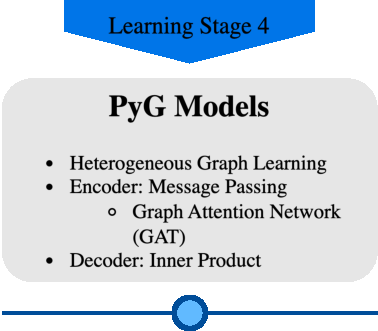
\includegraphics[width=\linewidth]{GNN/imgs/LearningStage4.pdf}
\end{minipage}

\end{frame}

%========================================================================================================================================================

\begin{frame}[fragile]
\begin{itemize}
\frametitle{Heterogeneous Graph Learning}
\setbeamertemplate{itemize items}[ball]

\item \textbf{Heterogeneous Graph Learning} refers to any graph-based neural network learning on a graph with more than two vertex or edge types.

\vspace{0.3cm}

\item Standard Message Passing GNNs (MP-GNNs) can not trivially be applied to heterogeneous graph data, as vertex and edge features from different types can not be processed by the same functions due to differences in feature type.

\vspace{0.3cm}

\item To automatically convert a homogeneous GNN model to a heterogeneous GNN model by making use of:

\lstinputlisting[basicstyle=\ttfamily\fontsize{4.5}{5.5}\selectfont,firstline=8, lastline=8]{GNN/code/main.py}

\end{itemize}
\end{frame}

%========================================================================================================================================================

\begin{frame}[fragile]
\frametitle{Case Study: Heterogeneous Graph Learning}
\setbeamertemplate{itemize items}[ball]

\hspace{3cm}
\begin{minipage}[c]{0.4\textwidth}
    \hspace{1cm}
    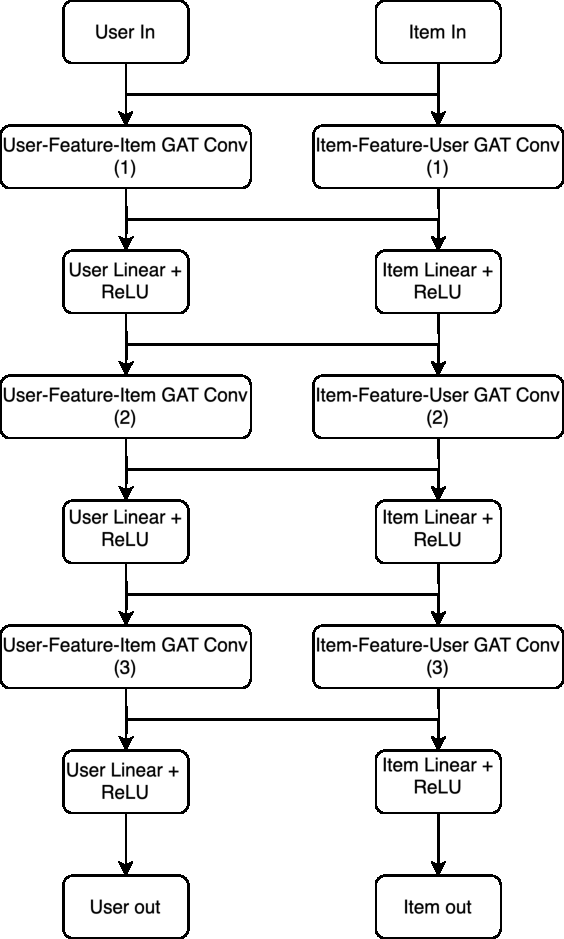
\includegraphics[width=\linewidth]{GNN/imgs/HeteroLearning.pdf}
\end{minipage}

\end{frame}

%========================================================================================================================================================

\begin{frame}[fragile]
\begin{itemize}
\frametitle{Graph Attention Network (GAT)}
\setbeamertemplate{itemize items}[ball]

\item The "Graph Attention Networks" research paper was first published in October 30th, 2017.

\vspace{0.3cm}

\begin{minipage}[c]{\linewidth}
    \hspace{1.5cm}
    
\includegraphics[width=0.7\linewidth]{GNN/imgs/gat.png}
\end{minipage}

\vspace{0.3cm}

\item The main idea is to compute the hidden representations of each vertex in the
graph, by attending over its neighbors, following a self-attention strategy.

\end{itemize}
\end{frame}

%========================================================================================================================================================

\begin{frame}[fragile]
\begin{itemize}
\frametitle{(1) GAT Layer: Linear Layer}
\setbeamertemplate{itemize items}[ball]

\item We begin by applying a shared
linear transformation, parameterized by a weight matrix $\textbf{W}$ on all of the vertex features $\textbf{h} = \{\overrightarrow{h_{1}},\overrightarrow{h_{2}},...,\overrightarrow{h_{N}} \}$:

\begin{center}
    \item[] $\textbf{W}\overrightarrow{h_{i}}, \textbf{W}\overrightarrow{h_{j}}$
\end{center}

\end{itemize}
\end{frame}

%========================================================================================================================================================

\begin{frame}[fragile]
\begin{itemize}
\frametitle{(1) Case Study: Linear Layer}
\setbeamertemplate{itemize items}[ball]

\item For recommendations systems, we apply two distinct shared linear transformations, parameterized by weight matrices $\mathbf{W_{\text{user}}}$ and $\mathbf{W_{\text{item}}}$ on the sampled sets of bipartite vertex features $\mathbf{h_{\text{user}}} = \{\overrightarrow{h_{1}},\overrightarrow{h_{2}},...,\overrightarrow{h_{N}} \}$ and $\mathbf{h_{\text{item}}} = \{\overrightarrow{h_{1}},\overrightarrow{h_{2}},...,\overrightarrow{h_{M}} \}$:

\begin{center}
    \item[] $\mathbf{W_{\text{user}}}\overrightarrow{h}_{user_{i}}, \mathbf{W_{\text{user}}}\overrightarrow{h}_{user_{j}}$
    \vspace{0.3cm}
    \item[] $\mathbf{W_{\text{item}}}\overrightarrow{h}_{item_{i}}, \mathbf{W_{\text{item}}}\overrightarrow{h}_{item_{j}}$

\end{center}
\end{itemize}
\end{frame}

%========================================================================================================================================================

\begin{frame}[fragile]
\begin{itemize}
\frametitle{(1) Linear Layer: Code}
\setbeamertemplate{itemize items}[ball]

\item Initializing $\mathbf{W_{\text{user}}}$ and $\mathbf{W_{\text{item}}}$:

\lstinputlisting[basicstyle=\ttfamily\fontsize{4.5}{5.5}\selectfont,firstline=163, lastline=166]{GNN/code/gat_conv.py}

\item Applying linear transformation and reshaping into a tensor of size (Batch, Heads, Output Channels):

\lstinputlisting[basicstyle=\ttfamily\fontsize{4.5}{5.5}\selectfont,firstline=282, lastline=286]{GNN/code/gat_conv.py}

\item Note: 'Src' and 'Dst' refer to Source and Destination vertex features; in our bipartite graph these are user and item vertex features.

\end{itemize}
\end{frame}

%========================================================================================================================================================

\begin{frame}[fragile]
\begin{itemize}
\frametitle{(2) GAT Layer: Self-Attention}
\setbeamertemplate{itemize items}[ball]

\item Then, we perform self-attention on the vertices.

\vspace{0.2cm}

\begin{center}
    \item[] $\alpha_{i,j} = \frac{\exp\left(\mathrm{LeakyReLU}\left( \overrightarrow{\mathbf{a}}^{\top}
    [\mathbf{W}\overrightarrow{h_{i}}\|
    \mathbf{W}\overrightarrow{h_{j}}]
\right)\right)}
{\sum_{k \in \mathcal{N}_{i}}
\exp\left(\mathrm{LeakyReLU}\left(
\overrightarrow{\mathbf{a}}^{\top}
    [\mathbf{W}\overrightarrow{h_{i}}\|
    \mathbf{W}\overrightarrow{h_{j}}]
\right)\right)}$
\end{center}

\vspace{0.5cm}

\item The attention coefficients $\alpha_{i,j}$ indicate the importance of vertex j’s features to vertex i.

\end{itemize}
\end{frame}

%========================================================================================================================================================

\begin{frame}[fragile]
\begin{itemize}
\frametitle{(2) GAT Layer: Self-Attention}
\setbeamertemplate{itemize items}[ball]

\begin{columns}
\hspace{1cm}
\begin{column}{0.5\textwidth}
\begin{minipage}[c]{1\textwidth}
    \item The attention mechanism $\overrightarrow{\mathbf{a}}$ is a learnable parameter that is multiplied to the concatenation of the output of the previous linear layer.
    \vspace{0.3cm}
    \item  The output is then passed through a LeakyReLU activation with negative slope 0.2, and a softmax normalization across all neighbors.
\end{minipage}
\end{column}
\hspace{2cm}
\begin{column}{0.6\textwidth}
\begin{minipage}[c]{\linewidth}
    \hspace{-1cm}
    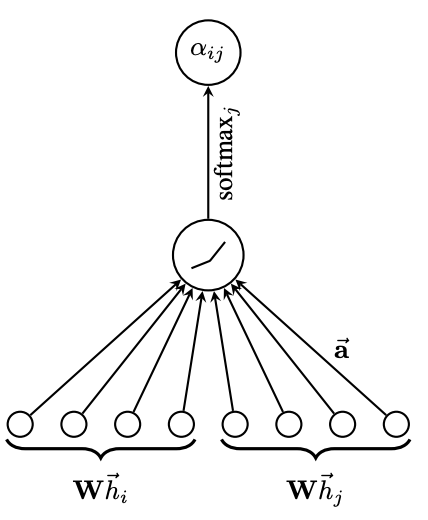
\includegraphics[width=0.6\linewidth]{GNN/imgs/self-attention.png}
\end{minipage}
\end{column}
\end{columns}

\end{itemize}
\end{frame}

%========================================================================================================================================================

\begin{frame}[fragile]
\begin{itemize}
\frametitle{(2) Case Study: Self-Attention}
\setbeamertemplate{itemize items}[ball]

\item For recommendation systems, we have two different attention coefficients calculated in the same manner:

\vspace{0.3cm}

\begin{center}
    $\alpha_{\text{user}_{i,j}} = \frac{\exp\left(\mathrm{LeakyReLU}\left( \overrightarrow{\mathbf{a}}_{\text{user}}^{\top}[\mathbf{W}_{\text{user}}\overrightarrow{h}_{\text{user}_{i}}\|\mathbf{W}_{\text{user}}\overrightarrow{h}_{\text{user}_{j}}]\right)\right)}{\sum_{k \in \mathcal{N}_{i}}\exp\left(\mathrm{LeakyReLU}\left( \overrightarrow{\mathbf{a}}_{\text{user}}^{\top}[\mathbf{W}_{\text{user}}\overrightarrow{h}_{\text{user}_{i}}\|\mathbf{W}_{\text{user}}\overrightarrow{h}_{\text{user}_{j}}]\right)\right)}$
\end{center}

\vspace{0.3cm}

\begin{center}
    $\alpha_{\text{item}_{i,j}} = \frac{\exp\left(\mathrm{LeakyReLU}\left( \overrightarrow{\mathbf{a}}_{\text{item}}^{\top}[\mathbf{W}_{\text{item}}\overrightarrow{h}_{\text{item}_{i}}\|\mathbf{W}_{\text{item}}\overrightarrow{h}_{\text{item}_{j}}]\right)\right)}{\sum_{k \in \mathcal{N}_{i}}\exp\left(\mathrm{LeakyReLU}\left( \overrightarrow{\mathbf{a}}_{\text{item}}^{\top}[\mathbf{W}_{\text{item}}\overrightarrow{h}_{\text{item}_{i}}\|\mathbf{W}_{\text{item}}\overrightarrow{h}_{\text{item}_{j}}]\right)\right)}$
\end{center}

\end{itemize}
\end{frame}

%========================================================================================================================================================

\begin{frame}[fragile]
\begin{itemize}
\frametitle{(2) Self-Attention: Code}
\setbeamertemplate{itemize items}[ball]

\item Initializing $\overrightarrow{\mathbf{a}}_{\text{user}}$ and $\overrightarrow{\mathbf{a}}_{\text{item}}$:

\lstinputlisting[basicstyle=\ttfamily\fontsize{4.5}{5.5}\selectfont,firstline=168, lastline=170]{GNN/code/gat_conv.py}

\item These parameters are then passed through glorot intializer:

\lstinputlisting[basicstyle=\ttfamily\fontsize{4.5}{5.5}\selectfont,firstline=199, lastline=200]{GNN/code/gat_conv.py}

\item Applying self-attention mechanism on previous output:

\lstinputlisting[basicstyle=\ttfamily\fontsize{4.5}{5.5}\selectfont,firstline=308, lastline=312]{GNN/code/gat_conv.py}

\end{itemize}
\end{frame}

%========================================================================================================================================================

\begin{frame}[fragile]
\begin{itemize}
\frametitle{(2) Self-Attention: Code}
\setbeamertemplate{itemize items}[ball]

\item Sampled self-attention coefficients are collected according to edge index:

\end{itemize}

\vspace{0.3cm}

\begin{columns}
\begin{column}{0.5\textwidth}
\hspace{2cm} $\alpha_{\text{user}_{i,j}}$
\lstinputlisting[basicstyle=\ttfamily\fontsize{3.5}{4.5}\selectfont,firstline=77, lastline=91]{GNN/code/edge_updater.py}
\end{column}
\begin{column}{0.5\textwidth}
\hspace{2cm} $\alpha_{\text{item}_{i,j}}$
\lstinputlisting[basicstyle=\ttfamily\fontsize{3.5}{4.5}\selectfont,firstline=94, lastline=107]{GNN/code/edge_updater.py}
\end{column}
\end{columns}

\end{frame}

%========================================================================================================================================================

\begin{frame}[fragile]
\begin{itemize}
\frametitle{(2) Self-Attention: Code}
\setbeamertemplate{itemize items}[ball]

\item These sampled attention coefficients are summed $\alpha_{user_{i,j}}+\alpha_{item_{i,j}}$ to emulate concatenation operator $\|$

\vspace{0.3cm}

\lstinputlisting[basicstyle=\ttfamily\fontsize{4.5}{5.5}\selectfont,firstline=367, lastline=369]{GNN/code/gat_conv.py}

\vspace{0.3cm}

\item LeakyReLU activation with negative slope 0.2, and a softmax normalization across all neighbors:

\lstinputlisting[basicstyle=\ttfamily\fontsize{4.5}{5.5}\selectfont,firstline=380, lastline=381]{GNN/code/gat_conv.py}

\end{itemize}
\end{frame}


%========================================================================================================================================================

\begin{frame}[fragile]
\begin{itemize}
\frametitle{(3) GAT Layer: Aggregation}
\setbeamertemplate{itemize items}[ball]

\item Once obtained, the normalized attention coefficients are used to compute a linear combination of the features corresponding to them, to serve as the final output features for every vertex:

\vspace{0.5cm}

\begin{center}
    \item[] $\overrightarrow{h_{i}}^{'} = \sum_{j \in \mathcal{N}_{i}} \alpha_{i,j} \textbf{W}\overrightarrow{h_{j}} $
\end{center}

\end{itemize}
\end{frame}

%========================================================================================================================================================

\begin{frame}[fragile]
\begin{itemize}
\frametitle{(3) Aggregation: Case Study}
\setbeamertemplate{itemize items}[ball]

\item For recommendation systems, only user final outputs vertex features $\overrightarrow{h}_{\text{user}_i}^{'}$ are propagated:

\end{itemize}

\vspace{0.3cm}

\begin{center}
    $\overrightarrow{h}_{\text{user}_i}^{'} = \sum_{j \in \mathcal{N}_{i}} (\alpha_{user_{i,j}}+\alpha_{item_{i,j}}) \mathbf{W}_{\text{user}}\overrightarrow{h}_{\text{user}_j}$
\end{center}

\end{frame}

%========================================================================================================================================================

\begin{frame}[fragile]
\begin{itemize}
\frametitle{(3) Aggregation: Code}
\setbeamertemplate{itemize items}[ball]

\item User neighborhood vertices are collected by sampled edge index:

\vspace{0.3cm}

\hspace{4cm} $\mathbf{W}_{\text{user}}\overrightarrow{h}_{\text{user}_j}$
\lstinputlisting[basicstyle=\ttfamily\fontsize{4.5}{5.5}\selectfont,firstline=71, lastline=87]{GNN/code/propagate.py}

\end{itemize}
\end{frame}

%========================================================================================================================================================

\begin{frame}[fragile]
\begin{itemize}
\frametitle{(3) Aggregation: Code}
\setbeamertemplate{itemize items}[ball]

\item Self-attention coefficient $\alpha_{user_{i,j}}+\alpha_{item_{i,j}}$ is multiplied to the linear layer output $\mathbf{W}_{\text{user}}\overrightarrow{h}_{\text{user}_j}$

\lstinputlisting[basicstyle=\ttfamily\fontsize{4.5}{5.5}\selectfont,firstline=385, lastline=387]{GNN/code/gat_conv.py}

\item Lastly, the message is propagated to neighborhood vertices $\sum_{j \in \mathcal{N}_{i}}$
\lstinputlisting[basicstyle=\ttfamily\fontsize{4.5}{5.5}\selectfont,firstline=69, lastline=77]{GNN/code/resolver.py}

\end{itemize}
\end{frame}

%========================================================================================================================================================

\begin{frame}[fragile]
\begin{itemize}
\frametitle{(Optional 4) GAT Layer: Multi-Head Attention}
\setbeamertemplate{itemize items}[ball]

\item Multi-head attention is an optional addition to stabilize the learning process of self-attention:

\end{itemize}

\begin{columns}
\begin{column}{0.5\textwidth}
\begin{minipage}[c]{\linewidth}
\vspace{0.5cm}
\hspace{0.5cm}
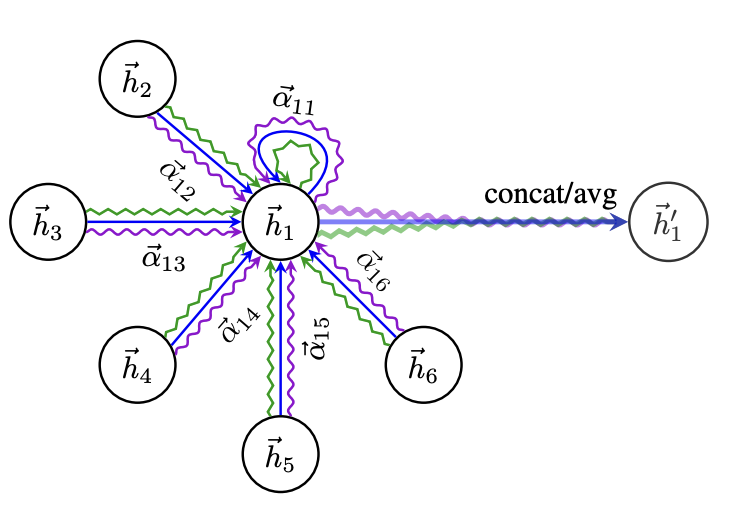
\includegraphics[width=1\linewidth]{GNN/imgs/multi-head.png}
\end{minipage}
\end{column}
\begin{column}{0.6\textwidth}
\begin{center}
    $\overrightarrow{h_{i}}^{'} = \frac{1}{k} \sum_{k=1}^{k} \sum_{j \in \mathcal{N}_{i}} \alpha_{i,j} \textbf{W}\overrightarrow{h_{j}}$
\end{center}
\end{column}
\end{columns}

\vspace{0.3cm}

\begin{itemize}
    \item We simply repeat the process $k$ times and average the messages.
\end{itemize}

\end{frame}

%========================================================================================================================================================

\begin{frame}[fragile]
\begin{itemize}
\frametitle{(Optional 4) Multi-Head Attention: Case Study}
\setbeamertemplate{itemize items}[ball]

\item For recommendation systems, only user final outputs vertex features $\overrightarrow{h}_{\text{user}_i}^{'}$ are propagated and averaged:

\vspace{0.3cm}

\begin{center}
    $\overrightarrow{h}_{user_{i}}^{'} = \frac{1}{k} \sum_{k=1}^{k} \sum_{j \in \mathcal{N}_{i}} (\alpha_{user_{i,j}}+\alpha_{item_{i,j}}) \textbf{W}_{user}\overrightarrow{h}_{user_{j}}$
\end{center}

\end{itemize}
\end{frame}

%========================================================================================================================================================

\begin{frame}[fragile]
\begin{itemize}
\frametitle{(Optional 4) Multi-Head Attention: Code}
\setbeamertemplate{itemize items}[ball]

\item To establish multi-head attention, one must set the 'concat' to False and specify the amount of heads:

\vspace{0.5cm}

\lstinputlisting[basicstyle=\ttfamily\fontsize{6.5}{7.5}\selectfont,firstline=343, lastline=346]{GNN/code/gat_conv.py}

\end{itemize}
\end{frame}

%========================================================================================================================================================

\begin{frame}[fragile]
\frametitle{GAT: Code}

\lstinputlisting[basicstyle=\ttfamily\fontsize{3.5}{4.5}\selectfont,firstline=60, lastline=80]{GNN/code/main.py}

\end{frame}


%========================================================================================================================================================

\begin{frame}[fragile]
\begin{itemize}
\frametitle{Inner Product Decoder}
\setbeamertemplate{itemize items}[ball]

\item Once we have our output vertex features for both user and item, we can decode them by performing a Hadamard multiplication and averaging across the
$N$ column dimension to get output $\overrightarrow{a}$:

\vspace{0.5cm}

\begin{center}
    \item[] $\overrightarrow{a} = \frac{1}{N} \sum_{N=1}^{N} \mathbf{h^{'}_{\text{user}}} \circ \mathbf{h^{'}_{\text{item}}}$
\end{center}

\end{itemize}
\end{frame}

%========================================================================================================================================================

\begin{frame}[fragile]
\frametitle{Inner Product Decoder: Code}
\setbeamertemplate{itemize items}[ball]

\lstinputlisting[basicstyle=\ttfamily\fontsize{6.5}{7.5}\selectfont,firstline=82, lastline=89]{GNN/code/main.py}

\end{frame}

%========================================================================================================================================================

\begin{frame}[fragile]
\frametitle{Loss Function}
\begin{itemize}

\item Finally, now that we have our output vector $\overrightarrow{a}$ we can calculate a mean squared error (MSE) with our target edge label vector $\overrightarrow{t}$:

\end{itemize}

\vspace{0.5cm}

\begin{center}
    $e = \frac{1}{n} \sum_{i=1}^{n} (\overrightarrow{t} - \overrightarrow{a})^2$
\end{center}

\vspace{0.5cm}

\begin{itemize}

\item In this manner, we can approximate edge label values to predict the existence of edges between users and items, or vice versa.

\end{itemize}
\end{frame}

%========================================================================================================================================================

\begin{frame}[fragile]
\frametitle{Loss Function: Code}

\lstinputlisting[basicstyle=\ttfamily\fontsize{6.5}{7.5}\selectfont,firstline=120, lastline=125]{GNN/code/main.py}

\end{frame}

%========================================================================================================================================================

\begin{frame}
\frametitle{}

\begin{minipage}[c]{0.8\textwidth}
    \hspace{1cm}
    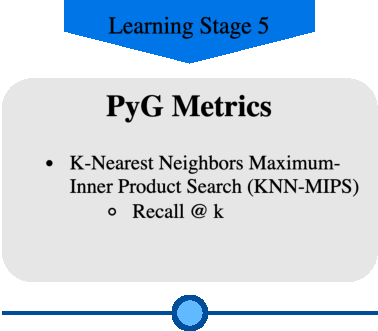
\includegraphics[width=\linewidth]{GNN/imgs/LearningStage5.pdf}
\end{minipage}

\end{frame}

%========================================================================================================================================================

\begin{frame}[fragile]
\begin{itemize}
\frametitle{Maximum Inner Product Search (MIPS)}

\item Given a collection of “database” vectors, $D = \{\overrightarrow{x}_{0}, \overrightarrow{x}_{1}, ..., \overrightarrow{x}_{d} \} \in S \subset R^{d}$ and a query $\overrightarrow{q} \in R^{d}$, \textbf{Maximum Inner Product Search} attempts to find a data vector $\overrightarrow{x_{*}}$ maximizing the inner product with the query:

\begin{center}
    \item[] $\overrightarrow{x_{*}} = argmax_{\overrightarrow{x} \in S} \ \overrightarrow{q}^T \overrightarrow{x} $
\end{center}

\end{itemize}
\end{frame}

%========================================================================================================================================================

\begin{frame}[fragile]
\begin{itemize}
\frametitle{Nearest Neighbor MIPS}
\setbeamertemplate{itemize items}[ball]

\item There are many variations of MIPS, one of them being \textbf{Nearest Neighbor MIPS} attempting to find a data vector $\overrightarrow{x_{*}}$ by minimizing over a distance function $\rho$:

\begin{center}
    \item[] $\overrightarrow{x_{*}} = argmin_{\overrightarrow{x} \in S} \ \rho(\overrightarrow{q}^T \overrightarrow{x}) $ \\~\\
    \underline{Intuition}: A neighbor of my neighbor is likely to be my neighbor.
\end{center}

\end{itemize}
\end{frame}

%========================================================================================================================================================

\begin{frame}[fragile]
\frametitle{K-Nearest Neighbor MIPS: Pseudocode}

\begin{minipage}[c]{1.4\textwidth}
    \vspace{-2cm} % This line adjusts the vertical position
    \hspace{-2.5cm}
    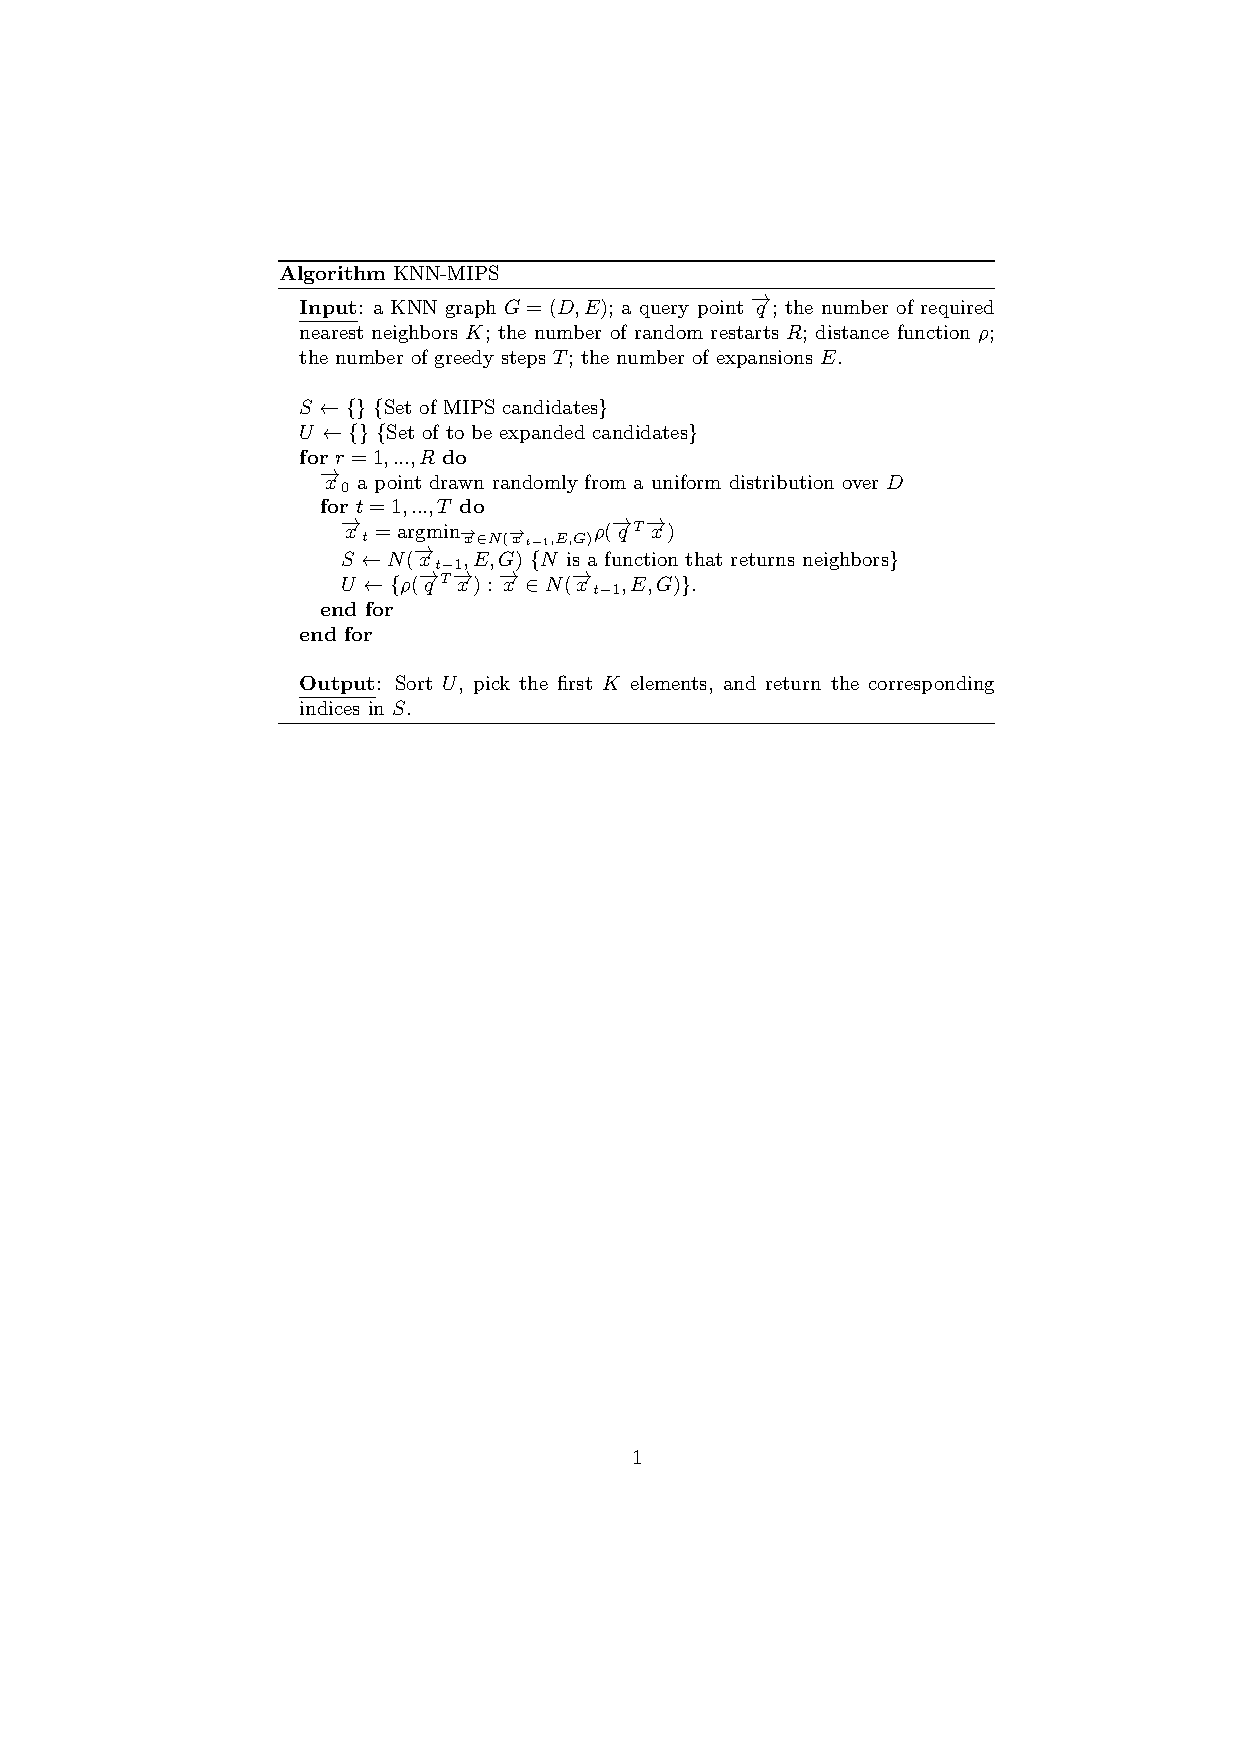
\includegraphics[width=\linewidth]{GNN/imgs/KNN-MIPS.pdf}
\end{minipage}

\end{frame}

%========================================================================================================================================================

\begin{frame}[fragile]
\begin{itemize}
\frametitle{K-Nearest Neighbor MIPS: Visualization}

\item Suppose greedy steps $T = 2$, neighbors $K = 1$ and expansions $E = 3$

\vspace{0.4cm}

\begin{minipage}[c]{0.5\textwidth}
    % \vspace{-2cm} % This line adjusts the vertical position
    \hspace{2.5cm}
    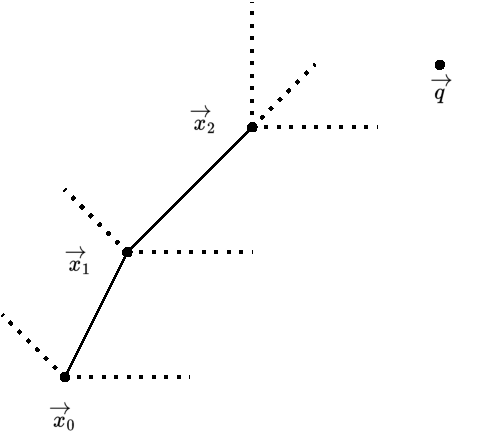
\includegraphics[width=\linewidth]{GNN/imgs/KNN-MIPSDRAW.pdf}
\end{minipage}

\end{itemize}
\end{frame}

%========================================================================================================================================================

\begin{frame}[fragile]
\begin{itemize}
\frametitle{K-Nearest Neighbors MIPS: Code}

\item At inference, we first calculate the embedding, or output features, for item vertices $\mathbf{h'}_{\text{item}}$

\lstinputlisting[basicstyle=\ttfamily\fontsize{4.5}{5.5}\selectfont,firstline=136, lastline=147]{GNN/code/main.py}

\item Then, we pass these item embedding vertices $\mathbf{h'}_{\text{item}}$ as our dataset vectors $D = \{\overrightarrow{x}_{0}, \overrightarrow{x}_{1}, ..., \overrightarrow{x}_{d} \}$

\item Note: positive embedding are passed as dataset vectors if we are utilizing negative sampling.

\end{itemize}
\end{frame}

%========================================================================================================================================================

\begin{frame}[fragile]
\begin{itemize}
\frametitle{K-Nearest Neighbors MIPS: Code}

\vspace{-0.3cm}

\item After passing dataset vectors, we calculate the embedding, or output features, for user vertices $\mathbf{h'}_{\text{user}}$

\lstinputlisting[basicstyle=\ttfamily\fontsize{4.5}{5.5}\selectfont,firstline=152, lastline=170]{GNN/code/main.py}

\vspace{-0.3cm}

\item We pass user embedding vertices $\mathbf{h'}_{\text{user}}$ as query vectors $Q = \{\overrightarrow{q}_{0}, \overrightarrow{q}_{1}, ..., \overrightarrow{q}_{d} \}$, $K$ neighbors and links to exclude.

\end{itemize}
\end{frame}

%========================================================================================================================================================

\begin{frame}[fragile]
\begin{itemize}
\frametitle{Recall @ K}
\setbeamertemplate{itemize items}[ball]

\item Recall at K calculates the fraction of relevant items among the top-K items recommended or retrieved.

\vspace{0.5cm}

\begin{center}
    \item[] $\text{Recall@K} = \frac{\text{Number of relevant items retrieved in top-K}}{\text{Total number of relevant items}}$
\end{center}

\vspace{0.5cm}

\item A high recall at K indicates that the system is good at retrieving relevant items in the top-K list.

\end{itemize}
\end{frame}

%========================================================================================================================================================

\begin{frame}[fragile]
\begin{itemize}
\frametitle{Recall @ K: Code}

\item We first initialize the class method with top-K amount of retrievals:

\lstinputlisting[basicstyle=\ttfamily\fontsize{6.5}{7.5}\selectfont,firstline=149, lastline=149]{GNN/code/main.py}

\vspace{0.5cm}

\item Then, we pass our matrix of predicted indices from our KNN-MIPS and corresponding edge index with excluded links:

\lstinputlisting[basicstyle=\ttfamily\fontsize{6.5}{7.5}\selectfont,firstline=172, lastline=174]{GNN/code/main.py}

\end{itemize}
\end{frame}

%========================================================================================================================================================

\begin{frame}
\frametitle{}

\begin{minipage}[c]{0.8\textwidth}
    \hspace{1cm}
    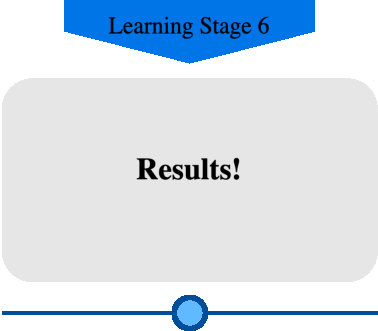
\includegraphics[width=\linewidth]{GNN/imgs/LearningStage6.pdf}
\end{minipage}
\end{frame}

%========================================================================================================================================================

\begin{frame}[fragile]
\begin{itemize}
\frametitle{Case Study: Simplified Movie Recommendation System}

\item Finally, we'll execute our GAT model with KNN-MIPS to assess whether recommending 'The Avengers' to Tim is feasible.

\vspace{0.5cm}

\begin{minipage}[c]{0.8\textwidth}
    \hspace{1cm}
    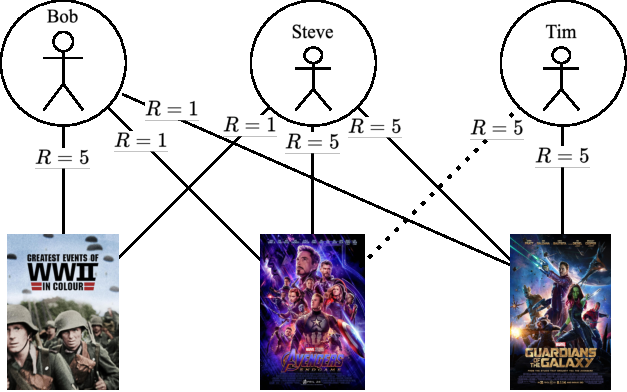
\includegraphics[width=\linewidth]{GNN/imgs/RecSysGraphLP.pdf}
\end{minipage}

\end{itemize}
\end{frame}

%========================================================================================================================================================

\begin{frame}[fragile]
\frametitle{Case Study: Hyperparameters}

\lstinputlisting[basicstyle=\ttfamily\fontsize{6.5}{7.5}\selectfont,firstline=13, lastline=28]{GNN/code/main.py}

\end{frame}

%========================================================================================================================================================

\begin{frame}[fragile]
\frametitle{Case Study: MSE Loss \& Recall @ 1}

\begin{columns}
\begin{column}{0.55\textwidth}
    \begin{minipage}[c]{\linewidth}
        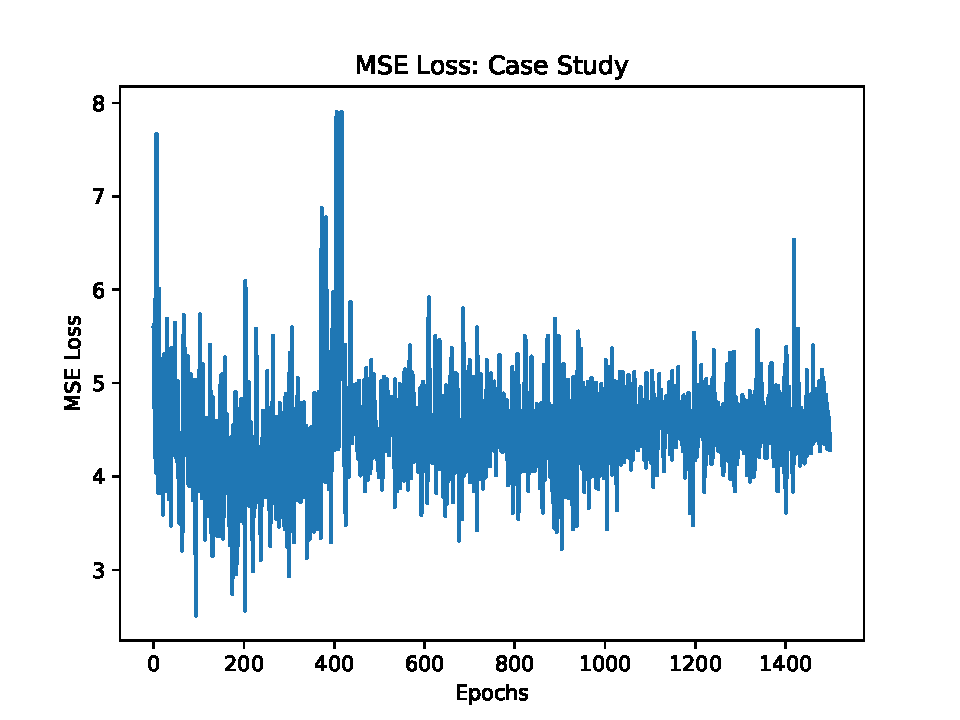
\includegraphics[width=\linewidth]{GNN/imgs/CaseStudyLoss.pdf}
    \end{minipage}
\end{column}
\begin{column}{0.55\textwidth}
    \begin{minipage}[c]{\linewidth}
        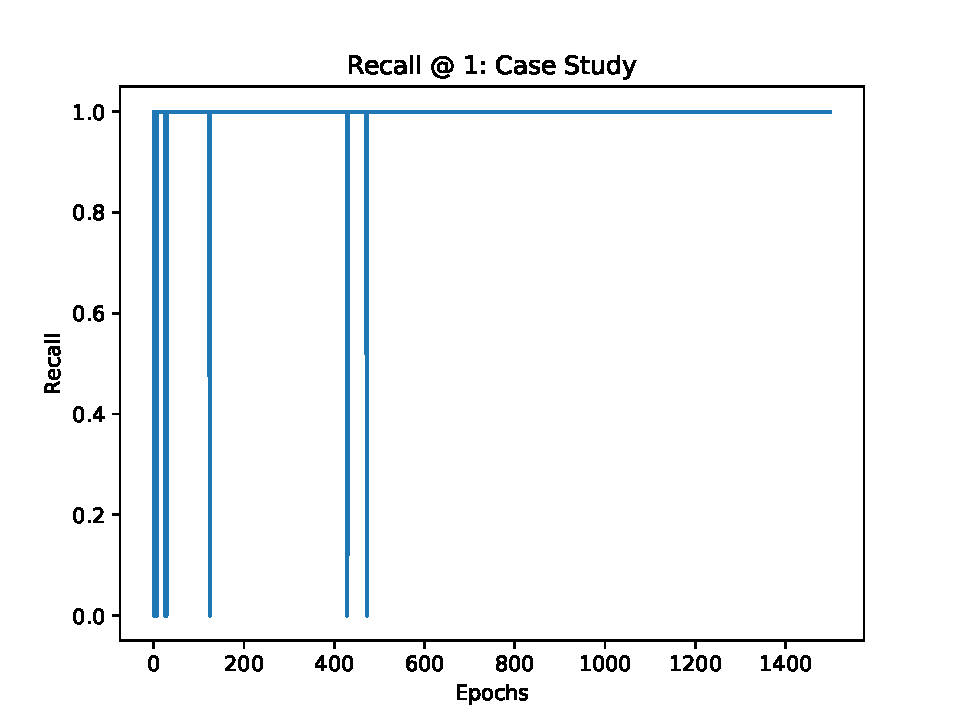
\includegraphics[width=\linewidth]{GNN/imgs/CaseStudyRecall.pdf}
    \end{minipage}
\end{column}
\end{columns}

\vspace{0.5cm}

\begin{itemize}
    \item Notice that after the first 500 epochs, the recommendation system converges to an optimal recommendation.
\end{itemize}

\end{frame}

%========================================================================================================================================================


\begin{frame}[fragile]
\begin{itemize}
\frametitle{References}
\setbeamertemplate{itemize items}[ball]

\item \href{https://pytorch-geometric.readthedocs.io/en/latest/}{\underline{PyG Documentation}}

\vspace{0.5cm}

\item \href{https://pytorch-geometric.readthedocs.io/en/latest/generated/torch_geometric.nn.conv.GATConv.html#torch_geometric.nn.conv.GATConv}{\underline{PyG GAT Documentation}}

\vspace{0.5cm}

\item \href{https://pytorch-geometric.readthedocs.io/en/latest/_modules/torch_geometric/nn/conv/gat_conv.html#GATConv}{\underline{PyG GAT Source Code}}

\vspace{0.5cm}

\item \href{https://www.ijcai.org/Proceedings/11/Papers/222.pdf}{\underline{KNN-MIPS Research Paper}}

\vspace{0.5cm}

\item \href{https://www.cse.cuhk.edu.hk/systems/hash/gqr/report/bob-slide.pdf}{\underline{KNN-MIPS Lecture}}

\vspace{0.5cm}

\item \href{https://github.com/twallett/GNN/blob/main/code/CaseStudy/main.py}{\underline{Code: Case Study - Simplified Movie Recommendation System}}

\end{itemize}
\end{frame}

%========================================================================================================================================================

\end{document} 